% Created 2023-10-20 Fri 09:59
% Intended LaTeX compiler: pdflatex
\documentclass[t, 10pt, seahorse, bigger]{beamer}
\usepackage[utf8]{inputenc}
\usepackage[T1]{fontenc}
\usepackage{graphicx}
\usepackage{longtable}
\usepackage{wrapfig}
\usepackage{rotating}
\usepackage[normalem]{ulem}
\usepackage{amsmath}
\usepackage{amssymb}
\usepackage{capt-of}
\usepackage{hyperref}
\usetheme[height=20pt]{Rochester}
\usecolortheme{seahorse}
\author{Konstantinos Vasilakos}
\date{2023-10-19}
\title{Intelligent Beheamoths: live coding with Ltt}
\hypersetup{
 pdfauthor={Konstantinos Vasilakos},
 pdftitle={Intelligent Beheamoths: live coding with Ltt},
 pdfkeywords={},
 pdfsubject={},
 pdfcreator={Emacs 28.2 (Org mode 9.7)}, 
 pdflang={English}}
\begin{document}

\maketitle
\begin{frame}{Outline}
\tableofcontents
\end{frame}

DESCRIPTION: Live coding with networked music system using Neural Network's regression algorithm trained by multiple users and sonified using SuperCollider's custom made sound synthesis modules.
\section{The Idea}
\label{sec:orgffba941}
\begin{frame}[label={sec:org24a16af}]{The Interface}
The system is a client/server application and communicates with OSC with other sound design environment:
\begin{center}
\begin{figure}[htbp]
\centering
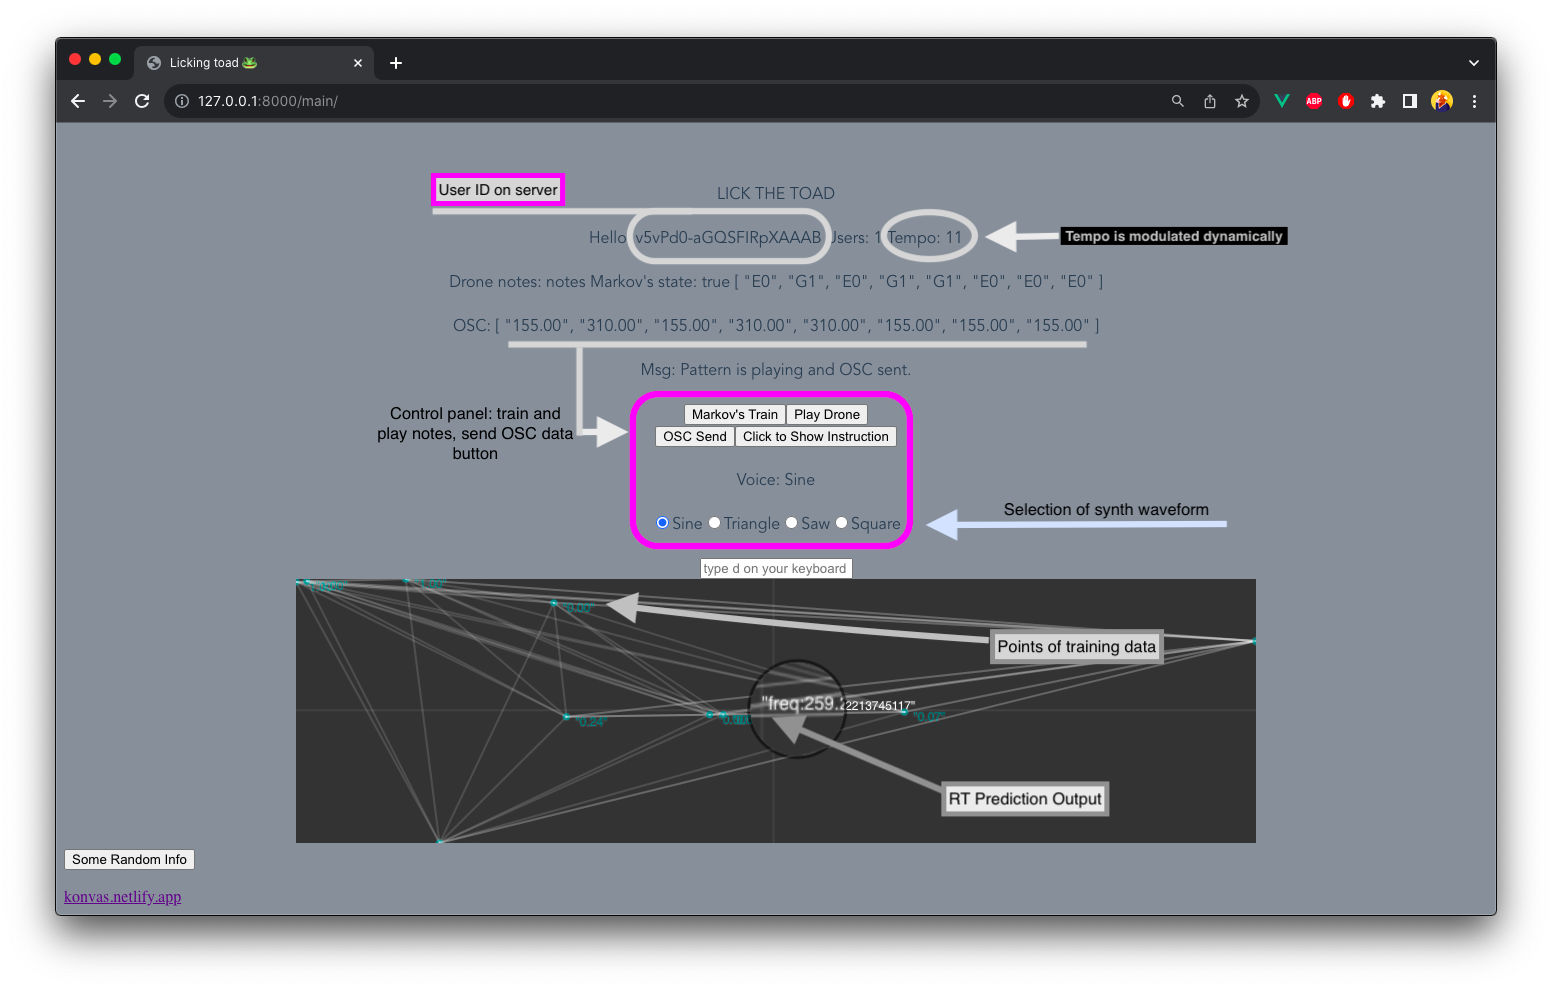
\includegraphics[width=.9\linewidth]{./screens/ltt-interface.png}
\caption{Ltt interface and control GUI.}
\end{figure}
\end{center}
\end{frame}
\section{Interaction}
\label{sec:org740015a}
\begin{frame}[label={sec:orge6d185e}]{Selection of Data on the Fly}
SuperCollider's part of the system supports selection of each event through the user's ID in a GUI.
\begin{center}
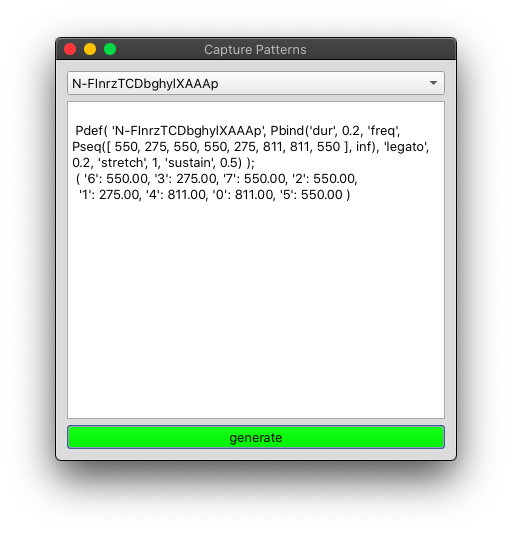
\includegraphics[height=0.5\textwidth]{./screens/sc-pop-up.png}
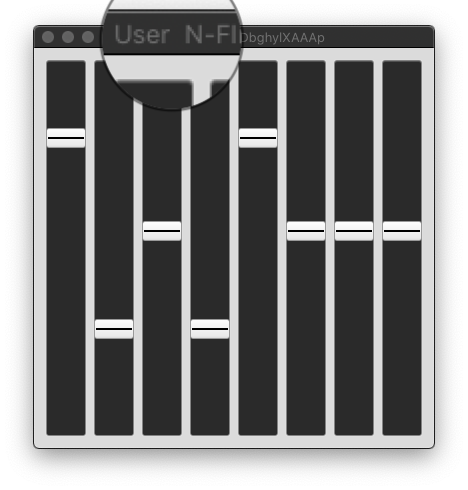
\includegraphics[height=0.5\textwidth]{./screens/sc-sliders.png}
\end{center}
\end{frame}
\section{Network Interaction}
\label{sec:org12835ec}
\begin{frame}[label={sec:org7881014}]{Interoperabillity}
[ "A0", "C4", "C4", "A0", "G2", "G2", "A0", "G2" ]
OSC:[ "214.00", "601.00", "601.00", "214.00", "428.00", "428.00", "214.00", "428.00" ]

The performance is shaped by the data of each user which is interpreted live while the performance unfolds. This way the sounds both from the decentralized domain of the user's together with the live electronics are creating an unpredictable sonic environment which enables the communication between audience and performer.
\end{frame}
\section{Sound Making}
\label{sec:orgda8bea6}
\begin{frame}[label={sec:org906865b}]{Performance method}
\begin{itemize}
\item The live coding performance is focussing on the real time sonification of the incoming data.
\item Each user is sending their data in an array of notes.
\item The coder is mapping this values in running processes with the help of streams and patterns of SuperCollider.
\end{itemize}
\end{frame}
\section{Live Coding}
\label{sec:org7fe8c37}
\begin{frame}[label={sec:org6eefa31},fragile]{Events Patterns and Streams}
 Performance elaborates using Patterns as random or sequential streams, and mapped to any sound parameter:
Examples of patterns include:
\(Prand, Pseq, Pser, Pxrand\)
and more\ldots{}

\begin{verbatim}
Pdef(\user_ID,
	Pbind(\dur, 0.1,
		\freq, Pseq([121.0, 220.0, 340.0, 280], inf)
	));
\end{verbatim}
\end{frame}
\section{Control from SC}
\label{sec:org312e4ec}
\begin{frame}[label={sec:orge8c45c9},fragile]{OSC Message Trigs}
 A small command line is also available from SC to set all users' new states of the Markov chain and trigger back new data.
\begin{verbatim}
n=NetAddr("localhost", 57122);
n.sendMsg('/kv', "markov_train");
n.sendMsg('/kv', "osc_trigger");
\end{verbatim}
\end{frame}
\section{Demo}
\label{sec:org084bc38}
\begin{frame}[label={sec:org9f7fb11}]{Live Coding.}
Live coding in SC -> play some now\ldots{}
\end{frame}
\section{Reflections}
\label{sec:orgf4a527d}
\begin{frame}[label={sec:org74df969}]{Points to consider}
The project aims to serve as an interconnector between coder and audience:
\begin{itemize}
\item Incoming data is the stimuli for real time arbitrary sonifications forming a dynamic soundscape.
\item An unpredictable sound result generated by the algorithm that is trying to connect the gaps by sending proximal values between X and Y coordinates from the user's device.
\item The input serves as the seeding input for a larger chain of processing and interconnection of modules, such as the Markovian chains and the machine learning modules bound together to offer a great paradox of a calculated surprise of unpredictable sonifications.
\end{itemize}
\end{frame}
\section{Development}
\label{sec:org4e18954}
\begin{frame}[label={sec:org0f4249d}]{Technical Details}
\begin{itemize}
\item Project is a client/server system encapsulating training/predictions.
\item Communication client/server is bound through WebSockets, and Express server.
\item Data from clients is using OSCJS library.
\item It is hosted locally with NodeJS and online -> \url{https://lick-the-toad.netlify.app/}
\begin{itemize}
\item Connection with users and OSC is supported only locally now.
\end{itemize}
\item Sound synthesis of clients is using Tone.js and Markov chains extension for JS.
\end{itemize}
\end{frame}
\end{document}